\chapter{Chapter 4: Thinking About Prototyping}

This chapter compiles lecture-quality study notes and comprehensive exam answers for \textbf{Unit IV: Prototyping} of the OE-EC803A syllabus, adhering strictly to the \textbf{MAKAUT Answer Writing Guidelines}.


\section{Section 1: Thinking About Prototyping \& The Cost vs. Ease Curve (Q4.2) [5M]}

\subsection{1. What is Prototyping in IoT?}
An IoT \textbf{prototype} is an early, experimental, and tangible manifestation of a connected device system, built to validate technical assumptions, test user interactions, and discover potential hardware/software integration flaws before committing to expensive mass production.

\subsection{2. The Cost vs. Ease of Prototyping Curve}
As an IoT project progresses from an abstract idea to a commercial product, the relationship between development cost, speed (ease of editing), and system flexibility changes dramatically.

\begin{figure}[H]
\centering
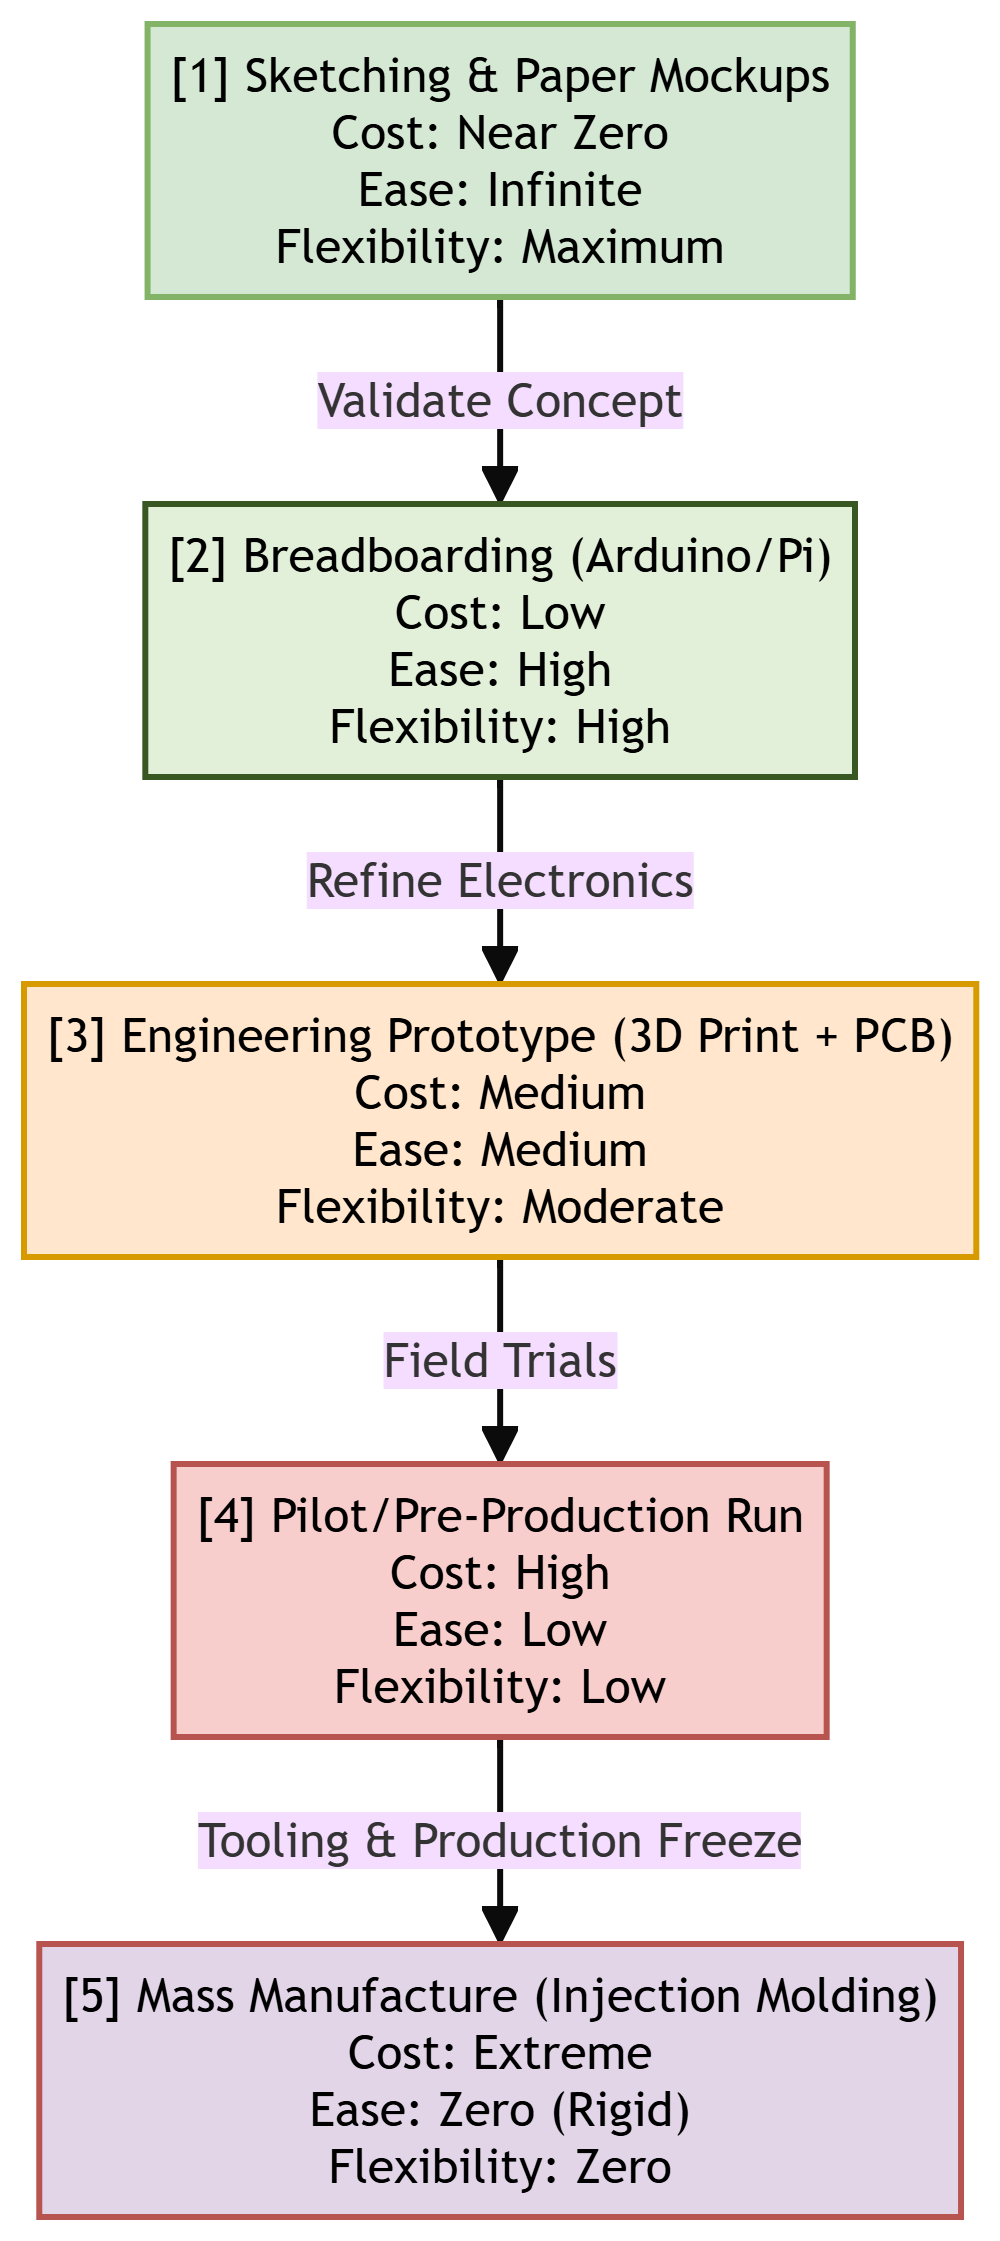
\includegraphics[width=0.75\textwidth,height=0.32\textheight,keepaspectratio]{../Images/chapter_04/cost_vs_ease.png}
\caption{Cost vs. Ease of Prototyping Curve}
\end{figure}

\subsubsection{The Five Progressive Phases of the Prototyping Curve:}
\begin{enumerate}
  \item \textbf{Phase 1: Sketching \& Paper Mockups:}
\end{enumerate}
    \textit{   }Characteristics:* Pen, paper, or simple cardboard structures.
    \textit{   }Cost:* Near zero.
    \textit{   }Ease \& Flexibility:* Infinite. Design edits can be done in seconds.
\begin{enumerate}
  \item \textbf{Phase 2: Breadboarding \& Sandbox (e.g., Arduino/Raspberry Pi):}
\end{enumerate}
    \textit{   }Characteristics:* Solderless breadboards, jumper wires, off-the-shelf development boards.
    \textit{   }Cost:* Low (a few dollars for chips/sensors).
    \textit{   }Ease \& Flexibility:* High. Changing connections or writing new firmware is fast and non-destructive.
\begin{enumerate}
  \item \textbf{Phase 3: Engineering Prototype (3D Printing \& Custom PCB):}
\end{enumerate}
    \textit{   }Characteristics:* Custom PCB layout, 3D-printed enclosure, soldered components.
    \textit{   }Cost:* Medium (tens to hundreds of dollars for custom boards and print runs).
    \textit{   }Ease \& Flexibility:* Moderate. Minor software tweaks are easy, but circuit re-design requires ordering new PCBs.
\begin{enumerate}
  \item \textbf{Phase 4: Pilot / Pre-Production Run:}
\end{enumerate}
    \textit{   }Characteristics:* Small batch run (e.g., 50–100 units) to test assembly pipelines and field deployment.
    \textit{   }Cost:* High. Custom tooling and manual testing setups are required.
    \textit{   }Ease \& Flexibility:* Low. Hardware is frozen; only software updates can be made.
\begin{enumerate}
  \item \textbf{Phase 5: Mass Production:}
\end{enumerate}
    \textit{   }Characteristics:* High-volume runs (thousands of units) using injection-molded casings and automated PCB assembly line testing.
    \textit{   }Cost:* Extreme upfront setup tooling costs (e.g., \$10,000+ for steel molds).
    \textit{   }Ease \& Flexibility:* Zero. Any design change at this stage is financially catastrophic.


\subsection{3. How Prototyping Bridges the Gap to Production}
Prototyping acts as a risk-mitigation bridge between a conceptual design and a final manufactured product. It achieves this by:
\begin{itemize}
  \item   \textbf{Identifying Hardware Vulnerabilities:} Discovering electrical noise, battery drain, or antenna interference issues in a low-risk environment.
  \item   \textbf{Firmware Logic Testing:} Isolating bugs in sensor sampling or connection reconnection logic before flashing thousands of devices.
  \item   \textbf{Validating Mechanical Fit:} Confirming that the PCB fits perfectly inside the plastic enclosure, and that connectors (e.g., USB port) align with outer cutouts.
  \item   \textbf{User Experience (UX) Feedback:} Testing if the physical size, button click feel, and light indicators are intuitive for the target user.
\end{itemize}


\section{Section 2: Open Source vs. Closed Source Paradigms (Q4.1) [5M]}

IoT developers must decide whether to build prototypes using \textbf{Open-Source} platforms or \textbf{Closed-Source (Proprietary)} commercial solutions.

\begin{figure}[H]
\centering
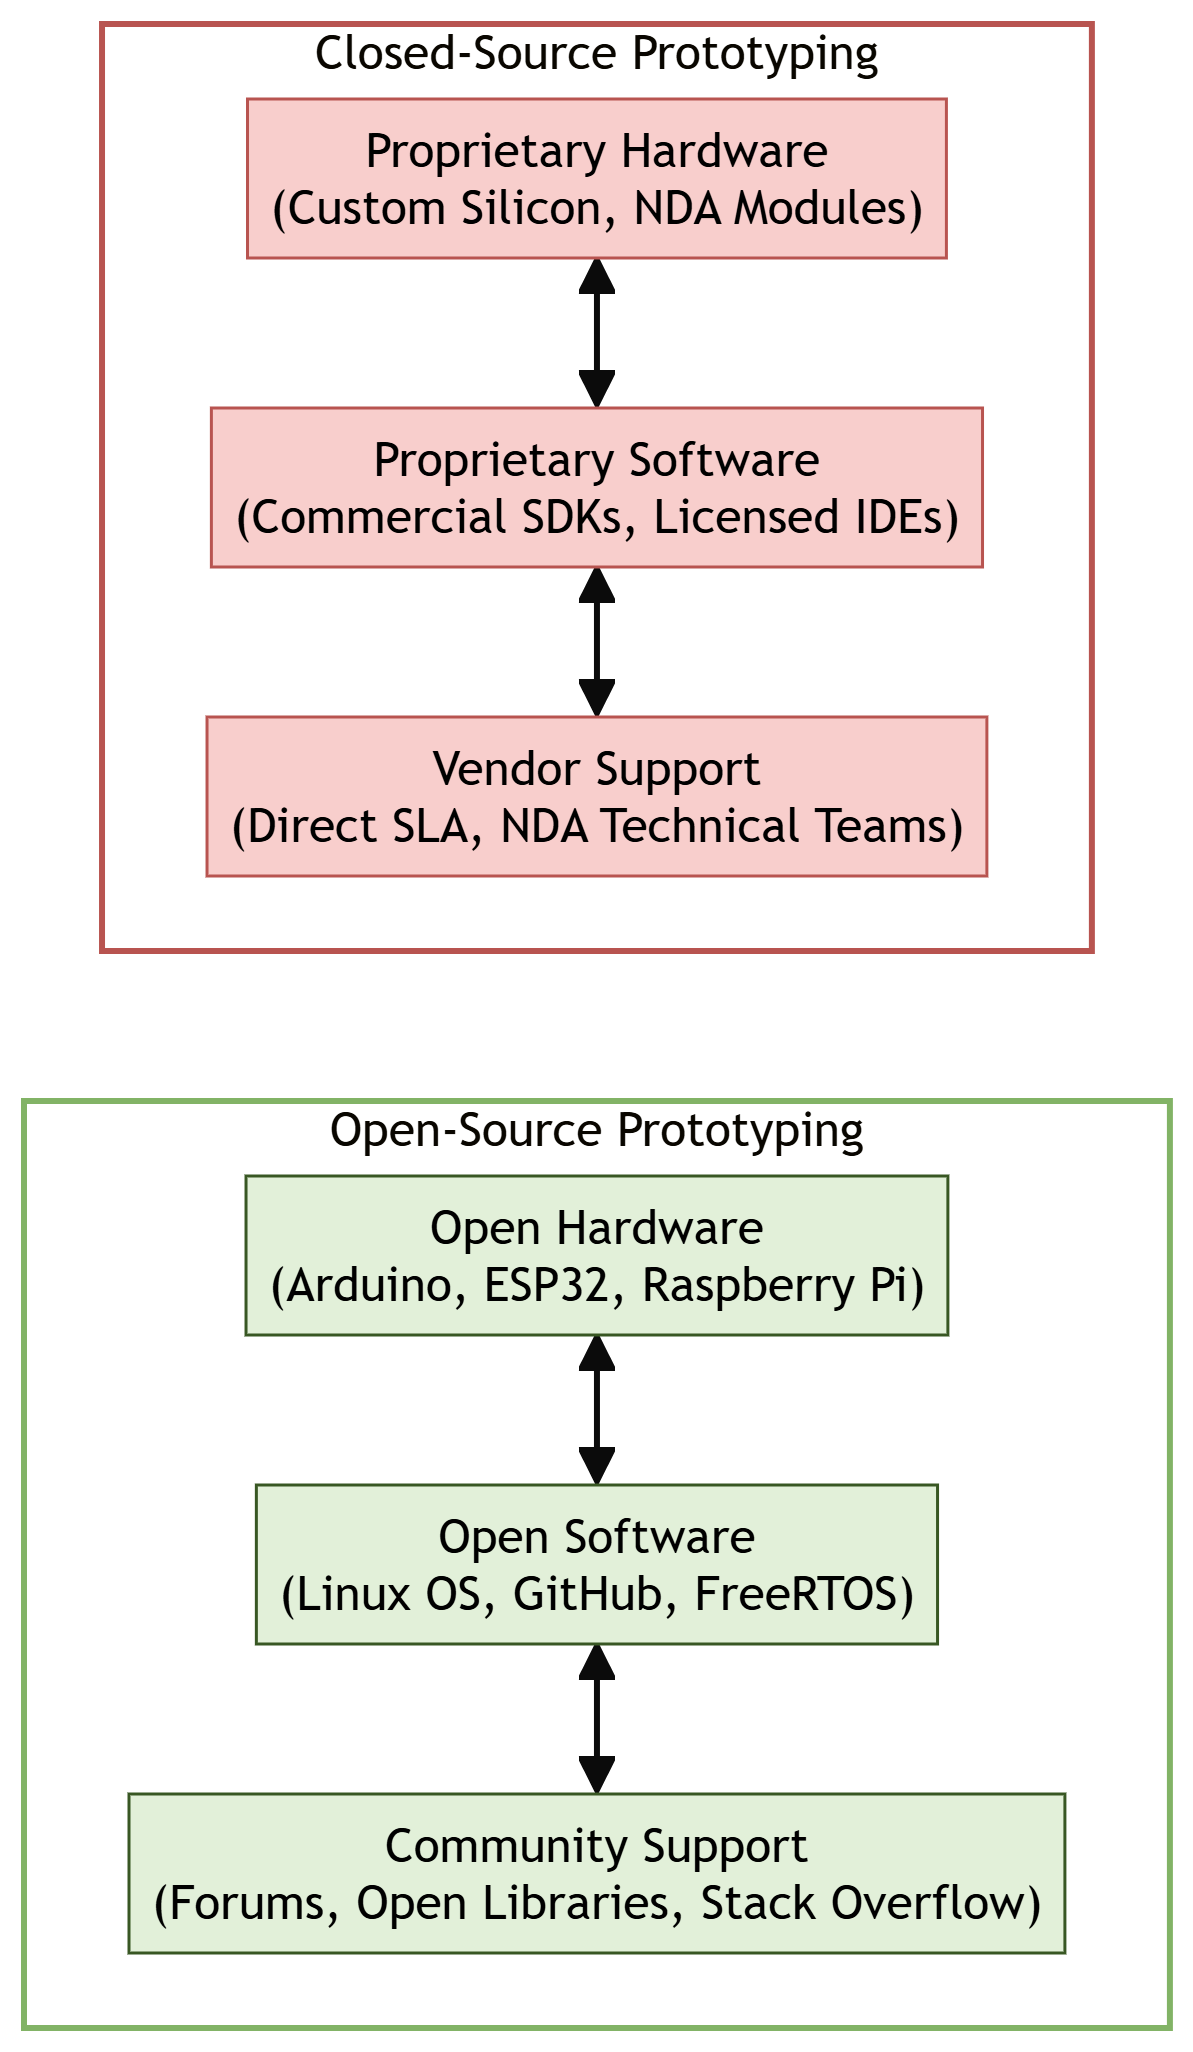
\includegraphics[width=0.75\textwidth,height=0.32\textheight,keepaspectratio]{../Images/chapter_04/open_vs_closed_source.png}
\caption{Open Source vs. Closed Source Ecosystems}
\end{figure}


\subsection{1. Comparison: Open Source vs. Closed Source in Prototyping}

\begin{table}[H]
\centering
\begin{tabular}{|p{\dimexpr 0.2\textwidth - 2\tabcolsep - 1.5\arrayrulewidth\relax}|p{\dimexpr 0.4\textwidth - 2\tabcolsep - 1.5\arrayrulewidth\relax}|p{\dimexpr 0.4\textwidth - 2\tabcolsep - 1.5\arrayrulewidth\relax}|}
\hline
Feature / Criteria & Open-Source Paradigm & Closed-Source (Proprietary) Paradigm \\
\hline
\textbf{Hardware Examples} & Arduino, Raspberry Pi, ESP32, BeagleBone. & Electric Imp, custom ASICs, locked-down OEM modules. \\
\hline
\textbf{Software/IDE} & Arduino IDE, GCC, FreeRTOS, Linux. & Keil, proprietary SDKs, vendor cloud compilers. \\
\hline
\textbf{Customizability} & Complete (full access to schematic files and code). & Limited (locked by vendor NDA or proprietary APIs). \\
\hline
\textbf{Upfront Cost} & Very low (often free software, cheap clone boards). & Higher (requires licenses, dev kits, seat keys). \\
\hline
\textbf{Development Speed} & Fast initial phase (millions of pre-written libraries). & Slower setup, but faster production transition. \\
\hline
\textbf{Support Channel} & Global community forums, GitHub issues. & Direct technical support, SLAs (Service Level Agreements). \\
\hline
\textbf{IP Protection} & Complex (often forces copyleft/open-sharing GPL). & High (protected under corporate licenses/secrets). \\
\hline
\end{tabular}
\end{table}


\subsection{2. Advantages and Disadvantages of Open Source}

\subsubsection{Advantages:}
\begin{enumerate}
  \item \textbf{Massive Pre-Existing Libraries:} Access to millions of free code libraries on GitHub for almost any sensor, bypassing the need to write drivers from scratch.
  \item \textbf{No Vendor Lock-In:} If a microcontroller chip becomes unavailable, the system can be adapted to another vendor since the schematics and toolchain are open.
  \item \textbf{Low Barrier to Entry:} Hobbyists and startups can build functional prototypes with minimal capital.
\end{enumerate}

\subsubsection{Disadvantages:}
\begin{enumerate}
  \item \textbf{Lack of Formal Support:} If a library has a critical bug, there is no vendor to call; you must rely on community goodwill or patch it yourself.
  \item \textbf{License Compliance Risks:} Accidentally mixing GPL-licensed code in commercial firmware can force a company to open-source its proprietary logic.
  \item \textbf{Inconsistent Documentation:} Community-supported platforms often suffer from outdated or incomplete documentation.
\end{enumerate}


\subsection{3. Advantages and Disadvantages of Closed Source}

\subsubsection{Advantages:}
\begin{enumerate}
  \item \textbf{Guaranteed Quality \& Support:} Direct access to technical engineers and Service Level Agreements ensures bugs are resolved rapidly.
  \item \textbf{Optimized for Production:} Vendor-managed modules often come pre-certified (e.g., FCC/CE rf certifications), saving months of testing.
  \item \textbf{High Intellectual Property (IP) Protection:} Keeps company code confidential, which is critical for securing venture capital.
\end{enumerate}

\subsubsection{Disadvantages:}
\begin{enumerate}
  \item \textbf{High Costs:} Licensing fees and proprietary developer seats can be prohibitively expensive.
  \item \textbf{Vendor Dependency:} If the vendor goes bankrupt or shuts down its cloud services, your IoT product becomes useless.
  \item \textbf{Inflexibility:} Inability to modify internal register states or custom-configure hardware parameters.
\end{enumerate}


\section{Section 3: Sketching, Familiarity, and Community (Q4.3) [5M]}

Successful rapid prototyping in IoT relies on three human-centric pillars: \textbf{Sketching}, \textbf{Familiarity}, and \textbf{Tapping into the Community}.


\subsection{1. The Role of "Sketching" in Early Prototyping}
In IoT, \textbf{Sketching} is not limited to pencil drawing; it refers to the practice of building \textbf{low-fidelity, non-functional physical mockups} to explore concepts.
\begin{itemize}
  \item   \textbf{Pencil \& Paper Sketches:} Visualizing the physical shape of the device, user interface placement (screen, LEDs, buttons), and user flow diagrams.
  \item   \textbf{Cardboard \& Foam Modeling:} Rapidly cutting out cardboards to construct a 3D model of the device. This helps verify the scale, how it fits in a user’s hand, or how it mounts on a wall.
  \item   \textbf{Software UI Mockups:} Creating non-functional, clickable phone screens using tools like Figma to test the app interface.
  \item   \textbf{Key Advantage:} Allows designers to discard bad ideas in minutes before spending time writing code or designing circuits.
\end{itemize}


\subsection{2. The Role of "Familiarity" in Prototyping Speed}
\textbf{Familiarity} refers to the developer's experience with their chosen tools (programming language, microcontroller family, CAD software).
\begin{itemize}
  \item   \textbf{Reducing Cognitive Load:} Using a tool you already know (e.g., Arduino C/C++ or Python) eliminates the learning curve, allowing you to focus entirely on solving the prototype's core engineering problems.
  \item   \textbf{Rapid Iteration:} A familiar toolchain allows developers to write, upload, and test firmware updates in minutes.
  \item   \textbf{Avoid the "Perfection Trap":} During prototyping, the goal is speed, not elegant production-level optimization. Using familiar, slightly bloated, but functional platforms (like Raspberry Pi running Python) is preferred over writing raw, optimized assembly code for a new 8-bit chip.
\end{itemize}


\subsection{3. The Significance of "Tapping into the Community"}
The global IoT developer community is a powerful force multiplier for rapid prototyping.
\begin{itemize}
  \item   \textbf{Collaborative Problem Solving:} Utilizing online communities (e.g., Arduino Forums, Stack Overflow, Hackster.io, ESP32 forum) to find quick fixes for obscure hardware bugs or compiler errors.
  \item   \textbf{Leveraging Open Source Packages:} Incorporating tested code bases (e.g., PubSubClient for MQTT, Adafruit libraries for sensors) to save months of manual register configuration.
  \item   \textbf{Crowdsourced Hardware Verification:} Reviewing open hardware designs (e.g., Adafruit Feather designs) to understand correct decoupling capacitor placements and antenna layouts.
  \item   \textbf{Conclusion:} In IoT, you are rarely the first person to encounter a specific technical problem. Tapping into the community allows you to stand on the shoulders of giants to bring a prototype to life quickly.
\end{itemize}
